% !TEX root = ../thesis-example.tex
%

\section{Device and System Independent Personal Touchless User Interface for Multi-Display}
AS computing technology is continuously developing, more and more computing systems are integrated in different scenarios. Today, the conventional display technology is still the 2D display and the information from different systems is shown on different displays. The modern day operating room is a typical scenario with multi-displays, where the surgeon performs surgeries with the support of different medical systems that showcase patient information, physiological data, and medical images. It is generally accepted that numerous interactions must be performed by the surgical team to control the corresponding medical system to retrieve the desired information. Joysticks and hardware keys are still present in the operating room due to the disadvantages of mouse, and surgeons often communicate instructions to the surgical team when wanting information from a specific medical system. Inspired by the method in Chapter\ref{chap:4-PAST}, we propose a solution to give the user direct control of the various systems' displays using only a single user interface via personal pointing gesture. 

More medical systems are integrated inside the operating room (OR) for diagnosis and intraoperative navigation as medical technology is continuously developing. \figurename{\ref{fig:4-PointingOR:ORScenario}} showcases the photo of a modern day operating room at Klinikum der Universit\"at M\"unchen - Campus Gro{\ss}hadern that consists of six unique displays for different medical information output.
Surgeons rely on these medical systems to capture, browse, and manipulate patient information, physiological data, and medical images, but the current control input of these systems is still mouse, keyboard, touch screen, and joystick. To interact with these medical systems and their control inputs, the user has to press either a physical/virtual button using their own finger or a visual cursor controlled by another device.
Yet, one of the most important rules in the OR is to maintain a strict boundary between what is sterile and what is not \cite{OHara2014a}. A sterile processing of the input devices is impossible; hence the surgeons cannot directly touch these input devices after they are scrubbed and gloved. However, research shows that the surgeon \underline{needs} to directly control the medical systems to mentally `get to grips' to what is going on, something which is not achievable by proxy \cite{Johnson2011a}. Giving the surgeon direct control of the interaction of different medical systems while maintaining sterility within the operating room has captured the imagination of many research groups and different solutions have been proposed.
In the operating room, the proposed user interface allows the surgeon to personally perform touchless interaction with the various medical systems, switch effortlessly among them, all of this without modifying the systems' software and hardware.
\begin{figure} [htb]
	% Use the relevant command to insert your figure file.
	% For example, with the graphicx package use
	\includegraphics[width=1.0\textwidth]{figures/4-PointingOR/ORScenario.png}
	% figure caption is below the figure
	\caption{There are six displays in a normal operating room in Klinikum der Universit\"at M\"unchen - Campus Gro{\ss}hadern for different medical systems. The function of these displays are 1\&2: DICOM images from the archive or live video streaming from the handle grip camera; 3: Arthroscopy Monitor; 4: SAP Hospital Information System; 5: Ample monitor sharing the same screen as 1 or 2; 6: Fluoroscopy monitor.}
	\label{fig:4-PointingOR:ORScenario}       % Give a unique label
\end{figure}
%To achieve this, a wearable RGB-D sensor is mounted on the user's head for inside-out tracking of their finger with any of the systems' displays. Android devices with a special application are connected to the computers on which different systems are running, simulating a normal USB mouse and keyboard. When the user performs interaction using pointing gestures, the desired cursor position in the targeted system display, and gestures, are transformed into general events and then sent to the corresponding Android device. Finally, the application running on the Android devices generates the corresponding mouse or keyboard events according to the targeted system. Finally, the novel user interface was evaluated in a simulated operating room setting by 7 medical participants who performed several interactions with three diverse medical interfaces at vary distances from them.

\subsection{System Design \& Methods}
Contrary to the state of art, we propose a novel user interface that allows the user to \underline{personally} perform touchless interaction with the \underline{various}  systems, and switch effortlessly among them, all of this \underline{without modifying} the systems' software and hardware. The advantages are: 
\begin{description} [font=$\bullet$\scshape\bfseries]
	\item needs no modification of the software/hardware of the existing systems and does not need the medical software to be re-certified
	\item combines pointing with personal gesture command
	\item switches smoothly among different medical systems and operands
	\item offers multi-user, multi-system framework
\end{description}
%without access to the current applications, no work zone limited, smoothly and naturally switch between different the medical systems and operands, multi-user and multi-medical system framework, and combining pointing with personal gesture command. 
%mouse event to simple and gesture too complex. our method is very flexible 
%personal gesture define for different functions. Traditional method is mouse and find the target and click.
%switch between different users smoothly 
In the proposed user interface setup, a wearable RGB-D sensor is mounted on the user's head for inside-out tracking of their finger with any of the various systems' displays. Android devices with a special application are connected to the computers on which the medical systems are running, simulating a normal USB mouse and keyboard. 
After calibration, the surgeon's pointing gesture can be recovered by a computing device. The target position in the real world, the desired cursor position in the display, and the user's personal gestures, are detected and analyzed. The result is sent to the Android devices via WiFi. The application running on the Android system generates the corresponding mouse or keyboard events according to the targeted system allowing completion of the interaction. In essence, one personal user interface is conceived to control all displays in a scenario. In this chapter, the hardware design and evaluation is instantiated in a modern operating room. 

\subsubsection{Hardware Setup \& Calibration}
A wearable RGB-D sensor  and a wearable computing device for each surgeon are introduced according to Chapter \ref{section:4-PAST}, and an Android device for each medical system. The proposed hardware setup with one surgeon and one medical system is shown in  \figurename{\ref{fig:4-PointingOR:Hardware}}.
The wearable RGB-D sensor is connected to the computing device and the Android device is connected to the medical system simulating a normal USB mouse and keyboard. The computing and Android devices exchange information via a WiFi router. To simplify the display tracking task, a 2D marker plane is attached to each display.
\begin{figure}[htb]
	% Use the relevant command to insert your figure file.
	% For example, with the graphicx package use
	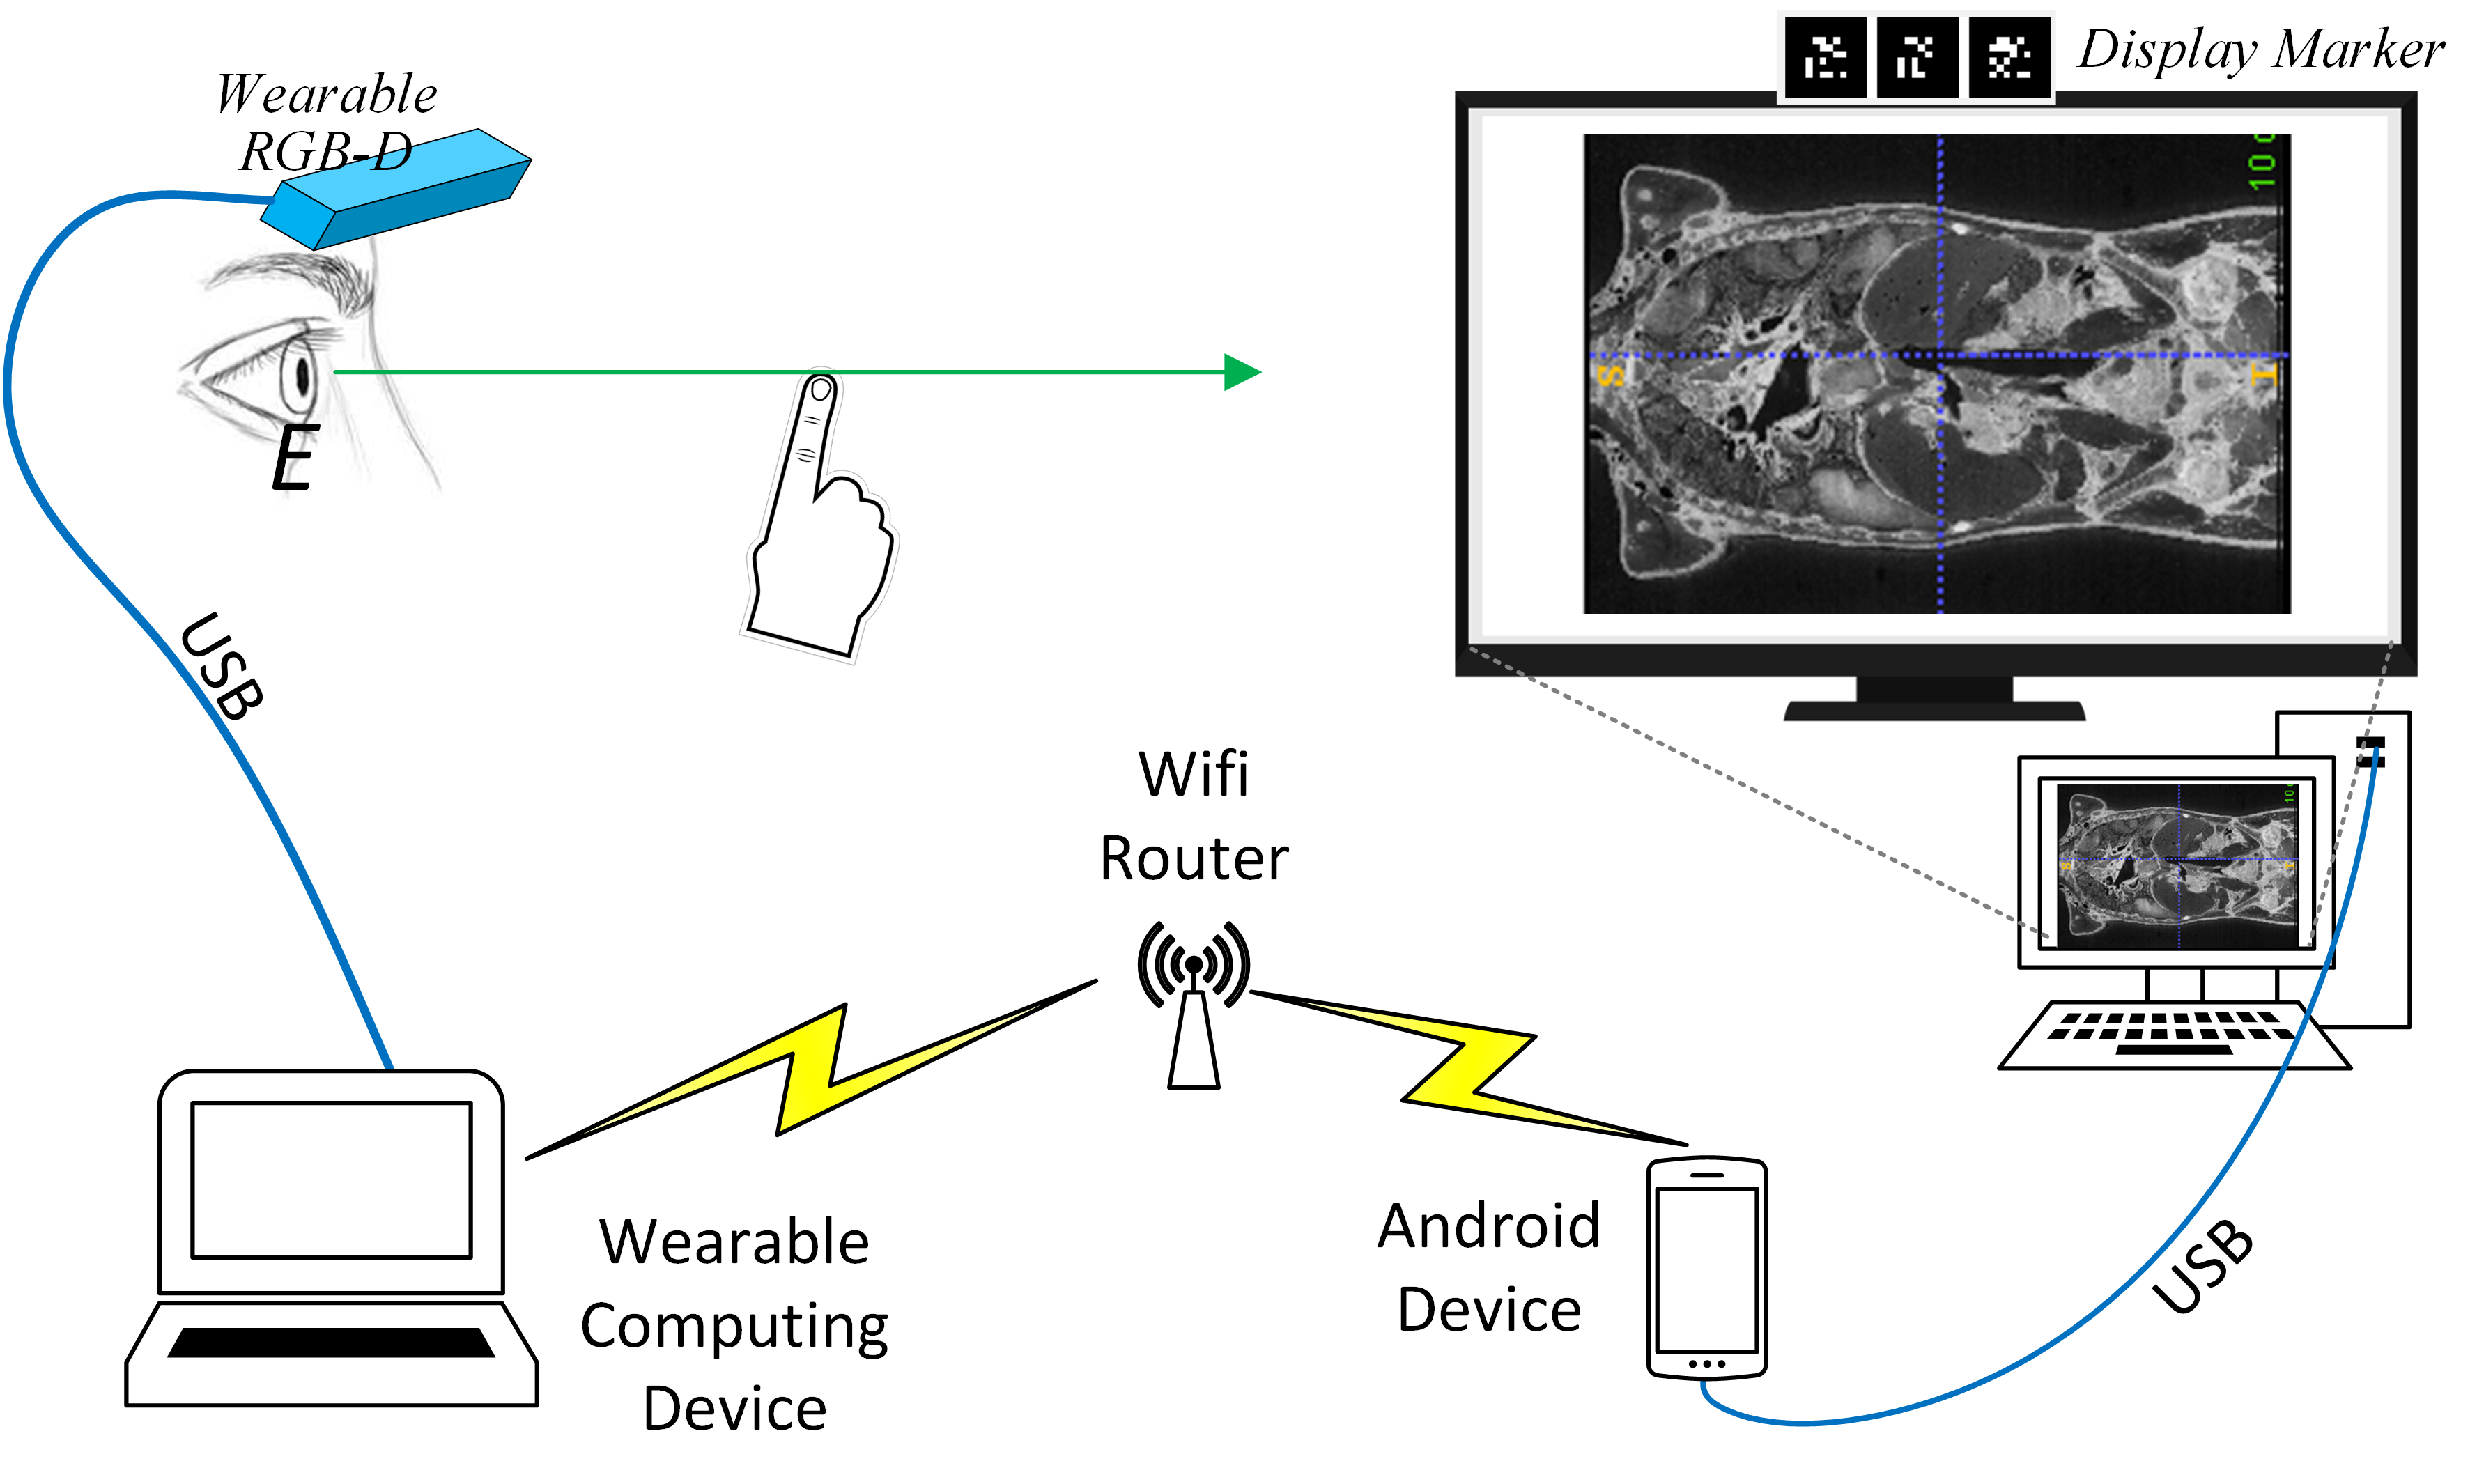
\includegraphics[width=1.0\textwidth]{figures/4-PointingOR/Hardware.png}
	% figure caption is below the figure
	\caption{The proposed hardware setup with a wearable RGB-D sensor, a wearable computing device, a medical system display, and an Android device.}
	\label{fig:4-PointingOR:Hardware}       % Give a unique label
\end{figure}

For our setup there are two parts that require calibration: i) the transformation between the display and its marker, and (ii) the user specific pointing gesture. The calibration methods are shown in \figurename{\ref{fig:4-PointingOR:Calibration}} and presented below.
\paragraph{Display with markers}
Without modifying any software/hardware of the existing medical systems, this calibration is performed with a marker printed on an A4 paper, as shown in  \figurename{\ref{fig:4-PointingOR:Calibration}}. 
The A4 paper is affixed closely next to the top-left corner of the display. Since the size of the A4 paper and the display are known, the translation of the printed marker relative to the display screen can be calculated. As the paper is very thin, the printed marker and the display are supposed to be coplanar. With the tracking information of the markers, the transformation matrix of the display relative to the display marker can be calculated. This one-time calibration process is performed offline for each display in the operating room. Then a configuration file is created for each display marker to describe which display it is attached to and which medical system is connected to this display. 
\begin{figure} [htb]
	\centering
	% Use the relevant command to insert your figure file.
	% For example, with the graphicx package use
	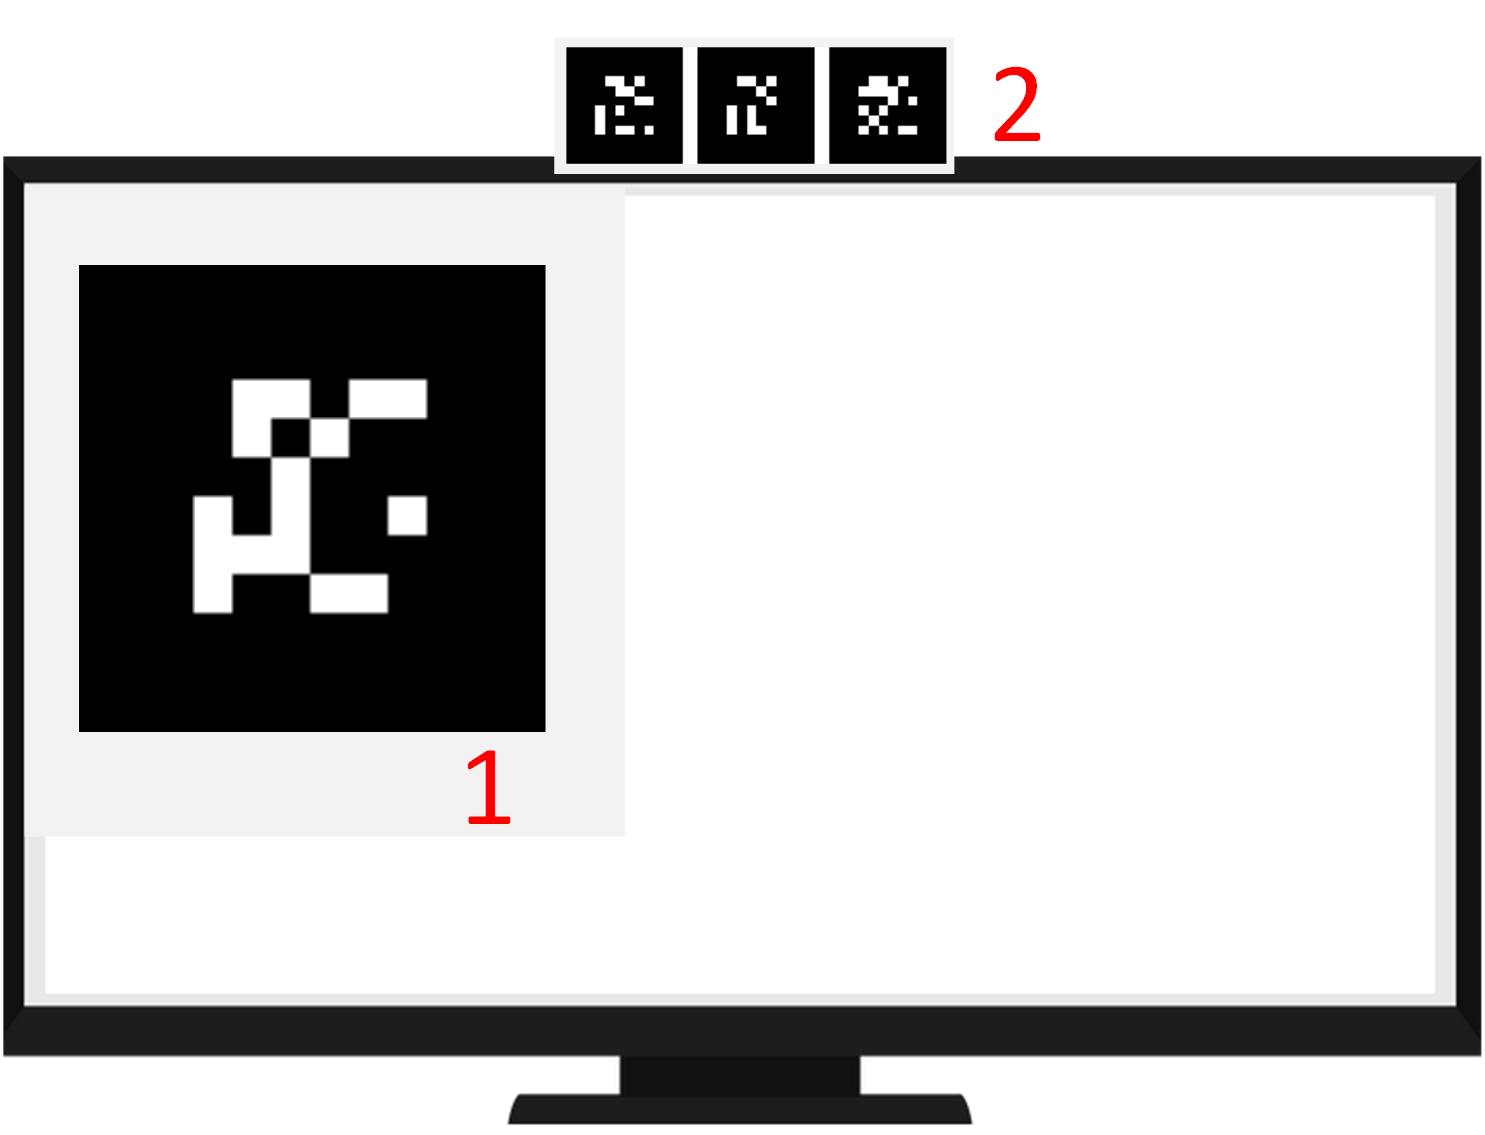
\includegraphics[width=0.5\textwidth]{figures/4-PointingOR/Calibration.png}
	% figure caption is below the figure
	\caption{Calibration methods: (a) A printed marker (1) is placed next to the right-top corner of the display to calculate the transformation matrix between the display marker (2) and the display. (b) Calibration of the user specific pointing gesture: the user is asked to point at several tracked targets $T_i$ using one finger and the pointing lines $L_i$ which pass through the fingertip $F_i$ and $T_i$ are collected.}
	\label{fig:4-PointingOR:Calibration}       % Give a unique label
\end{figure}
\paragraph{User specific pointing gesture}
In section \ref{sec:4-PAST:Methodology}, the objective of the proposed method is to calibrate and recover the user specific pointing geometry. The result of the calibration is the position of a virtual eye center $E$ for the user.
As shown in \figurename{ \ref{fig:4-PAST:PSATCalibration}, the target, $T_i$, is shown somewhere in the front of the user, who is then asked to perform a natural pointing gesture towards $T_i$ using one finger. The 3D positions of the fingertips $F_i$ and $T_i$ are collected through the wearable RGB-D sensor. The pointing line $L_i$ is defined such that it passes through $F_i$ and $T_i$. After sufficient pointing lines are collected, the intersection of the lines is calculated defining the user specific virtual eye-center $E$. After calibration the pointing geometry is recovered as $L_{i}$, going through $E$ and  $F_i$, when the pointing gesture is performed.

\subsubsection{System Framework}

\begin{figure} [htb]
	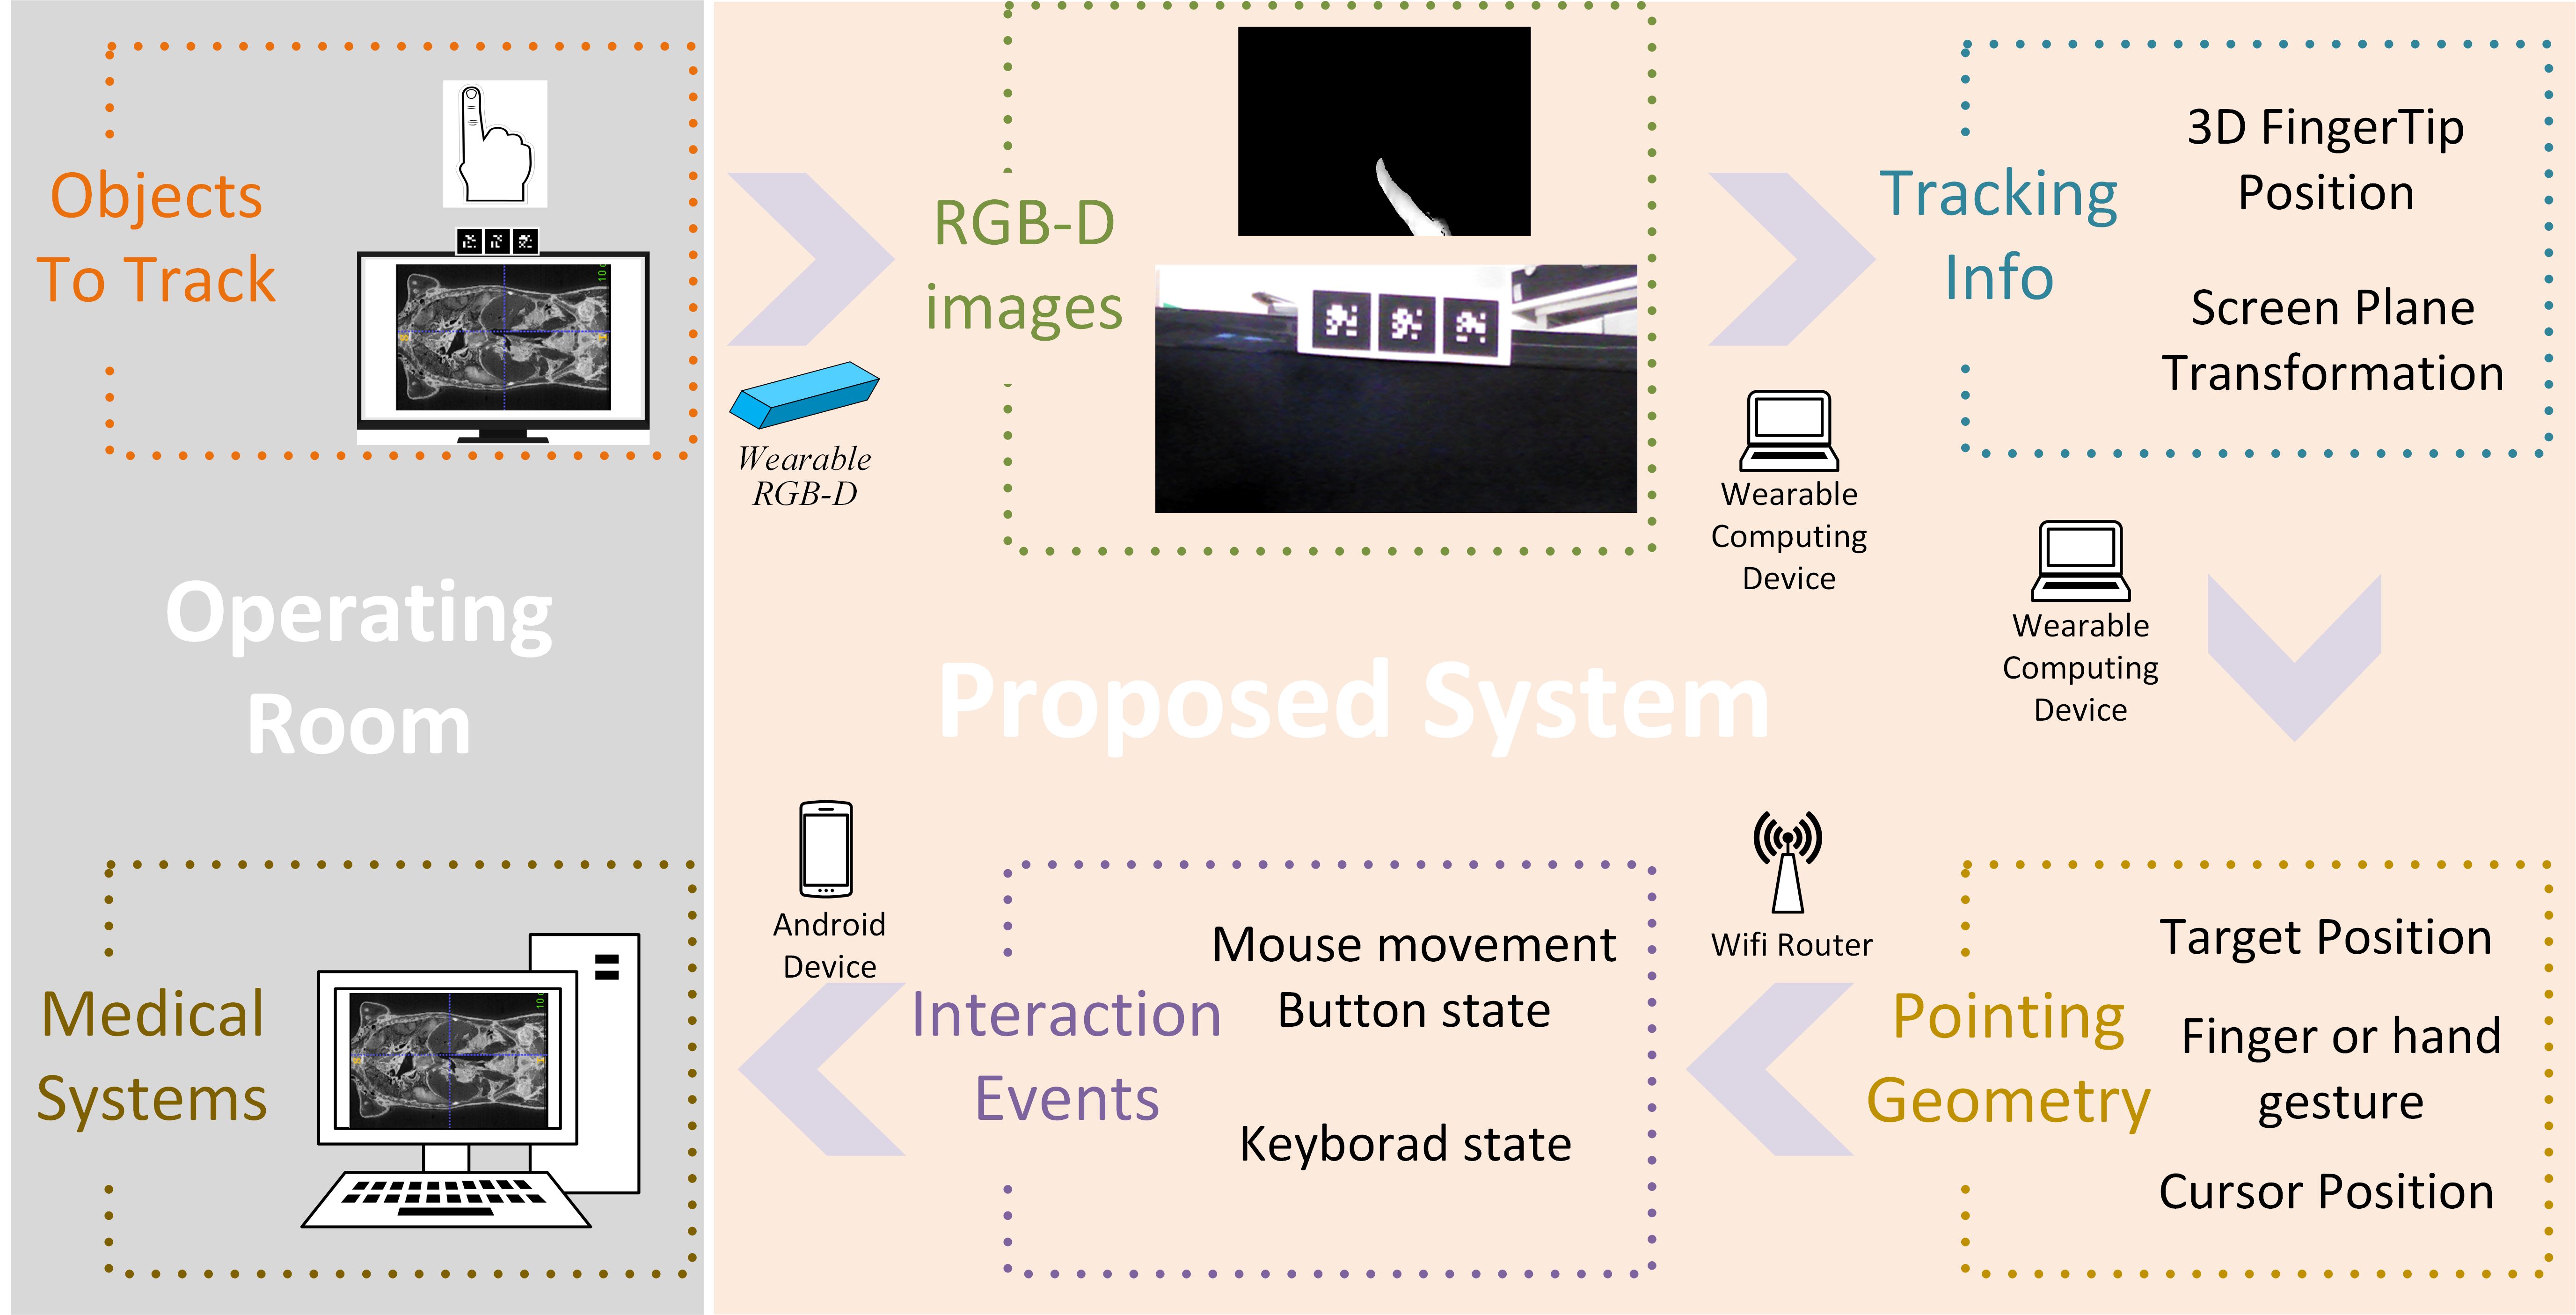
\includegraphics[width=1\textwidth]{figures/4-PointingOR/Workflow.png}
	\caption{The framework of the proposed system: Tracking information of objects in the OR after processing is used to control the medical systems. }
	\label{fig:4-PointingOR:Workflow}       % Give a unique label
\end{figure}
The system framework is shown in \figurename{\ref{fig:4-PointingOR:Workflow}}.
The left side shows the usual elements in the OR and the right side shows the data-flow of our user interface paradigm. When a surgeon performs interaction with a medical system, the display marker and fingertip can always be detected via the RGB-D sensor as it has a similar view as the surgeon. 
Through the following processing: \textit{Tracking Info}, \textit{Pointing Geometry}, and \textit{Interaction Events}, mouse and keyboard events are generated to control any medical systems.
\paragraph{Tracking Info} 
All the images are perceived via the wearable RGB-D sensor. Therefore, this is an inside-out tracking and does not require an external reference. The fingertip is detected from the depth image using 3D blob extraction and the display marker position is calculated via the color image.
\paragraph{Pointing Geometry}
Based on the calibration of ``User specific pointing gesture" and the tracking information,
the pointing geometry between the pointing direction and the display screen plane is recovered. The target position in real world and the desired cursor position on the screen can be calculated. We can also detect some predefined finger and hand gestures. Finally, all these information are transformed into general events and then sent to the corresponding Android device through UDP (User Datagram Protocol) connections. 
\paragraph{Interaction Events}
Two virtual devices are created in a Linux kernel to simulate USB mouse and keyboard when the Android device is connected to a computer. The two devices send normal initial signals to the host computer and are recognized as USB mouse and keyboard. The special application running on the Android system builds up a UDP connection with the computing devices to receive general events transformed from the pointing geometry and generates the corresponding mouse or keyboard events according to the current medical system. In our general design, all the interactions are implemented via the Android mouse or keyboard as the medical system is taken as a black box. However, the computing device could directly communicate with the medical system when this is allowed. 
\begin{figure} [htb]
	\includegraphics[width=1\textwidth]{figures/4-PointingOR/MultiUserMultiSystem.png}
	\caption{A setup with Multi-user Multi-system and the Android system structure. In this setup, there are two surgeons and two medical systems, one of which has two displays. }
	\label{fig:4-PointingOR:multiUserMultiSystem}       % Give a unique label
\end{figure}
During the Pointing Geometry stage, a personal configuration file could also be loaded to implement the multi-user case and personalized figure-pointing gestures. 
\paragraph{Multi-user Multi-system Scenario}
From \figurename{\ref{fig:4-PointingOR:multiUserMultiSystem}}, there can be more than one surgeon and more than one medical system in the operating room scenario. In the configuration file, each member of the surgical team is assigned a priority level according to his or her responsibility. When Android devices receive information from more than one computing device at the same time, they implement the mouse and keyboard event of the surgeon with higher priority level. This can solve the issues which arise when these systems are used in the context of an actual surgical procedure, including collaboration, engagement and disengagement. When there are more than one displays connected to a medical system, it still works well as the Android device knows which display is the desired one. Even when there is no display for a medical system, a display marker still can be positioned somewhere to simulate a virtual display, which is logically connected to the medical system. In this case, the surgeon can point at the display marker and perform interaction with the corresponding system.
\paragraph{Personalized Pointing Gesture}
Performing interactions requires two steps: i) choosing the target, and (ii) releasing the command. Through pointing gestures the surgeon can choose the target naturally via the pointing and immediately perform a finger or hand gesture to release the command. During the calibration procedure, the calibration of user pointing provides the characteristics of a user specific pointing geometry. In addition, since the pointing gesture is personal, pointing characteristics could be saved for each surgeon in order to recognize their gesture and map it to different commands.

\subsection{Evaluation \& Results}
The main goal of the user study is to answer the following questions: 
\begin{description}
	\item[1.] To what degree do the surgeon accept the interaction with multiple medical systems via our novel user interface?
	\item[2.] Do the surgeons find the system a viable alternative to the traditional indirect control of the medical systems and their displays in the modern day operation room?
\end{description}
Please note that we are not evaluating the gesture accuracy, but we are assessing the Android-based communication with the different systems. 
\subsubsection{Implementation}
\paragraph{Proposed system}
%todo{More detail about the Android App and the gesture design, Active box detection}
During the user study, the Intel \textit{Realsense} Creative camera was chosen as the wearable camera and Microsoft Surface 2 as the computing device, which was put in a backpack. The special Android application was installed on two Nexus 7 devices to simulate the USB mouse and keyboard for each medical system. 
\paragraph{Patient scenario}Anonymous patient is wheeled inside emergency room following a car accident. A CT was taken after neck trauma to rule out fractures. As no fractures were found but instability due to disc ligament tear was suspected, an MRI was carried out that confirmed it. Anonymous patient then went to surgery where C-arm fluoroscopy images were taken intraoperatively to alleviate problem via navigation.
\paragraph{Simulated medical systems}
The operating room was simulated in our laboratory with three displays showing CT, MRI, and C-arm fluoroscopy images. 
MicroDicom\cite{Tangcharoen2011} was used to visualize the C-arm fluoroscopy image in \textbf{display A}, InVesalius\cite{Moraes2012} was used to visualize the CT volume in \textbf{display B}, and MRI images were loaded directly in \textbf{display C}. The sizes of Monitor A, B, and C are 24 $''$, 42$''$ and 22$''$ and were placed at different locations and distances from the surgeon, as shown in \figurename{\ref{fig:4-PointingOR:ORSEnvironment}}. The interactions to be performed with these medical images were defined similar as those performed inside the modern day operating rooms:
\begin{description}
	[align=right,style=nextline,leftmargin= 0.3\linewidth,labelsep=\parindent,font=\normalfont]
	\item [Fluoroscopy image:] up-down flip , left-right flip
	\item [CT \& MRI images:] go through the images in axial, sagittal, coronal\\ zoom in/out in axial, sagittal, coronal
\end{description}
\begin{figure}
	% Use the relevant command to insert your figure file.
	% For example, with the graphicx package use
	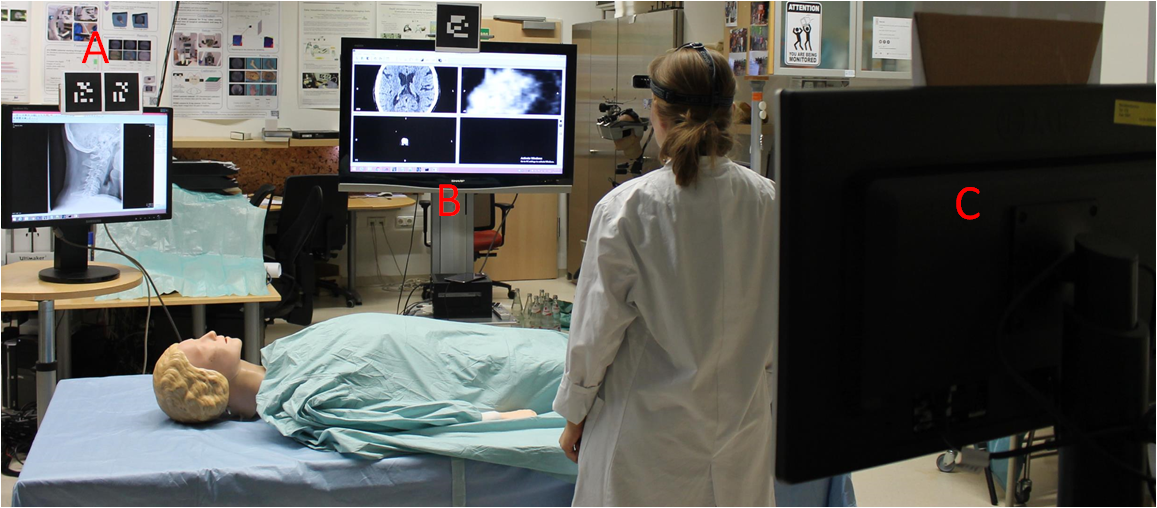
\includegraphics[width=1.0\textwidth]{figures/4-PointingOR/Displays.png}
	% figure caption is below the figure
	\caption{There are three displays in the simulated scenario, where the C-arm fluoroscopy , CT, and MRI images are shown in display A, B, and C, respectively.}
	\label{fig:4-PointingOR:ORSEnvironment}       % Give a unique label
\end{figure}
\paragraph{Mouse and keyboard events}
Going through the images in axial, sagittal, and coronal in InVesalius\cite{Moraes2012} is done by clicking at the image window and rotating the mouse wheel. Zooming is triggered by pressing the right mouse button down and moving the mouse up or down. To flip images using MicroDicom [19], it is necessary to trigger it by pressing buttons `Ctrl' with `F' or `H' at the same time. 

\textit{Proposed interaction}- The intersection between the pointing direction and the screen plane is calculated as the cursor position, and a mouse click function is generated when the surgeon points to a new image window via his or her finger. Mouse wheel events are generated to go through the CT \& MRI data when the surgeon is pointing towards the InVesalius image window and moving their finger left or right in the middle of the window. For zooming, the `right mouse button press down' event is triggered when moving their finger up or down. The button event `Ctrl+H' is generated for left-right flipping of the C-arm fluoroscopy image when the surgeon is pointing towards the MicroDicom and moving their finger left or right. Similarly, the `Ctrl+F' button event is triggered to flip up-down the C-arm fluoroscopy images when surgeons move their finger up or down in right side of the window.
\subsubsection{User study Design}
In order to answer the above questions, a qualitative user study was conducted with 7 participants (3 expert surgeons and 4 final year medical students). First, we introduced the concepts, user interface system, types of interactions, and experimental setting to the participants. Second, each participant put on the wearable RGB-D sensor and underwent a test period lasting 3 minutes to get comfortable with the initial calibration step and subsequent interactions. The distance of the displays to the participants are: display A-1.5 meters, display B-3 meters, and display C-1 meter.

The interaction sequence with the three different displays and data is as follows. Each participant was asked to visualize the CT images for neck fracture(s), browsing through the slices and magnifying specific regions within the slice in \textbf{display B}. Then, the participants were asked to either rotate their head or body to confirm the site of the ligament tear in the MRI images by browsing through the images and magnifying them to face \textbf{display C}. Finally, the participants looked at the C-arm fluoroscopy \textbf{display A} to flip the X-ray images correctly.

The following metrics were measured during the course of the experiments. First, we measured the total time in seconds for the participants to interact with the three displays. Then, following the user study, we had a short interview with each of the participants and they were asked to complete an adapted System Usability Scale (SUS) \cite{Brooke1996} questionnaire using a Five-point Likert scale (\textit{ 1-Strongly disagree, 2-Disagree, 3-Neither agree nor disagree, 4-Agree, 5-Strongly agree}). Lastly, the participants completed the NASA-TLX \cite{Hart2006}, which is a multi-dimensional scale ranked on 100 designed to obtain cognitive workload estimates from one or more operators while they are performing a task or immediately afterwards. The total workload is divided into six subscales that are represented as: \textit{Mental Demand, Physical Demand, Temporal Demand, Performance Effort, and Frustration}. The higher value from NASA-TLX means a higher cognitive workload.
\subsubsection{Results}
Although we did not have the same number of surgeons as students the measured average time to finish all the basic interactions with the three displays was 114$\pm$13 seconds for the medical students and 115$\pm$15 seconds for the experts. 
The results for the adapted SUS questionnaire are shown in \tablename{\ref{tb:4-PointingOR:questionnaire}}.
All responses were positive. The highest scores were credited to questions \#6 and \#11 which indicate that the participants would prefer our user interface over the existing ones in the operating rooms (4.4 $\pm$ 0.8), and that such user interface did not require a significant amount of learning (4.7 $\pm$ 0.4). The lowest scores were attributed to questions \#4 and \#10 which indicate that participants did not feel confident (3.9 $\pm$ 0.5) which did not allow for a subsequent smooth interaction. Finally, the result of NASA-TLX cognitive workload is shown in \figurename{\ref{fig:4-PointingOR:NASATLX}}. The highest workload occurred for \textit{Effort} and \textit{Performance} with average scores of 48\% and 49\% respectively. The participants did not have high cognitive workload for the remaining subscales with values ranging between 20\% and 33\%.
\begin{table}
	\caption{The Likert scale results of the usability questionnaire}
	\label{tb:4-PointingOR:questionnaire}
	\scriptsize
	\begin{center}
		\begin{tabular}{p{8cm}|p{1.2cm}}
			Questions & Scale \\
			\hline
			\textit{Q1:} The pointing gesture is intuitive for interaction. &  $4.1\pm0.7$ \\
			\textit{Q2:} It is very smooth to switch between different medical system. & $4.3\pm0.8$ \\
			\textit{Q3:} It is not complicated to get used to the system. & $4.1\pm0.7$ \\
			\textit{Q4:} The system feels responsive. & $3.4\pm0.7$\\
			\textit{Q5:} I  think the system is consistent. & $4.0\pm0.6$ \\
			\textit{Q6:} I prefer the proposed system instead of indirect interaction. & $4.4\pm0.8$ \\
			\textit{Q7:} The system is easy to use.& $3.9\pm0.9$ \\
			\textit{Q8:} I think that I would like to use this system. & $4.3\pm0.6$ \\
			\textit{Q9:} I would imagine that most people would learn to use this system very quickly. & $4.3\pm1.0$ \\
			\textit{Q10:} I felt very confident using the system. & $3.9\pm0.5$ \\
			\textit{Q11:} I didn't need to learn a lot of things before I could get going with this system & $4.7\pm0.4$
		\end{tabular}
	\end{center}
\end{table}
\begin{figure}
	\centering
	% Use the relevant command to insert your figure file.
	% For example, with the graphicx package use
	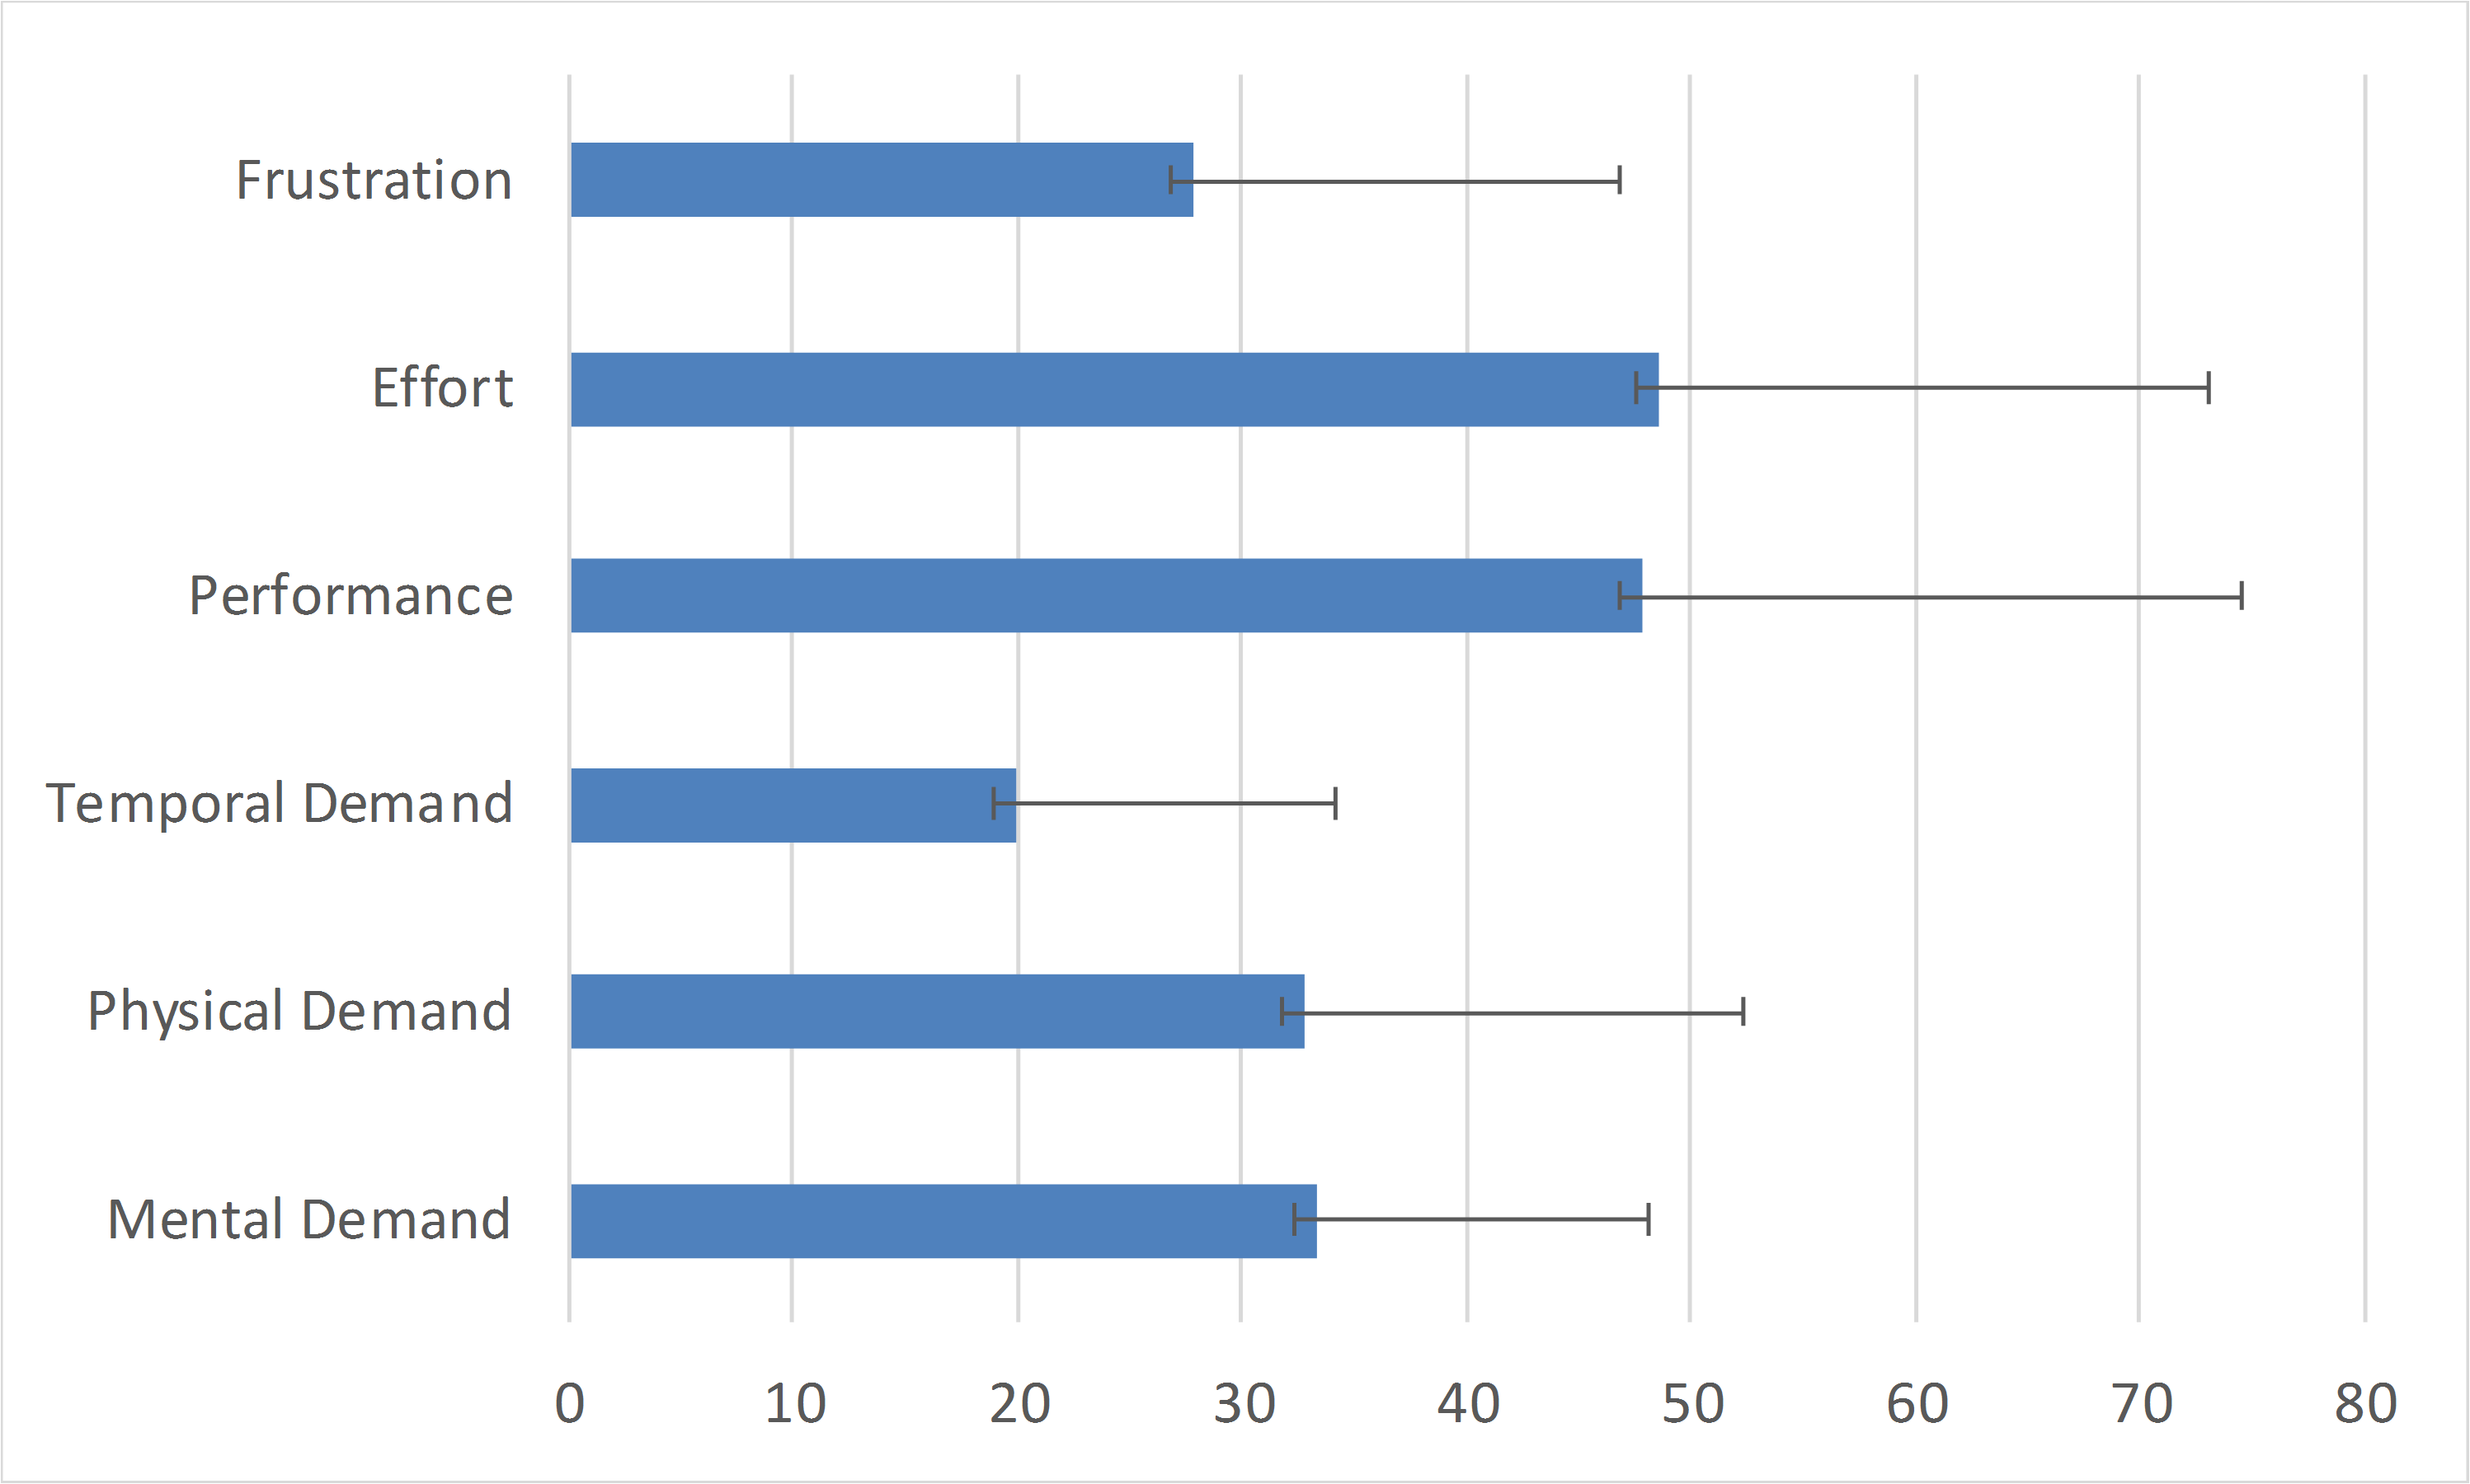
\includegraphics[width=0.7\textwidth]{figures/4-PointingOR/NASATLX.png}
	% figure caption is below the figure
	\caption{The results of NASA-TLX cognitive workload.}
	\label{fig:4-PointingOR:NASATLX}       % Give a unique label
\end{figure}

\subsection{Discussion \& Conclusion}%Outlook}
Like most new technologies, the learning curve for the participants needs to be considered when interpreting the results of our user study. As each of the 7 medical participants did not have any prior knowledge with our user interface, it was not surprising to note that there was no significant difference in the time required to complete the interactions.  It was also expected that participants did not feel confident using the user interface for the first time as seen from the adapted SUS results. This effect translated to the cognitive workload NASA-TLX with highest scores to the following questions:\textit{(Performance) How successful were you in accomplishing what you were asked to do?} and \textit{(Effort) How hard did you have to work to accomplish your level of performance?}

Albeit these short fallings, the vast majority of the results were positive. With consistent use of our UI, participants agreed that the potential impact of the proposed user interface compared to the traditional interfaces found in the operating room is clear. Our unique framework allows the surgeon to personally perform touchless interaction with the various medical systems at different locations and distances, switch effortlessly among them, all this without modifying the systems’ software and hardware. Comparing with the traditional methods our proposed framework is very general and can be adapted to multi-users and multi-displays. The objective of this paper was to present the main user interface paradigm, and not evaluate the accuracy of the different gestures for displays A-B-C.

In 2014, the authors in \cite{Pederson2010} provided insights and guidelines when developing user interfaces for the operating room. A key consideration is the physical location of surgeons when they need to interact with different medical systems. The patient table can be a crowded environment, with surgeons often in close proximity to other members of the surgical team. Not only can this affect a system’s approach to tracking but also impose constraints on the kinds of movement available for gesture design. In sterile practice, hand movements must be restricted to the area extending forward from the surgeon's torso between the hips and chest level. Moreover, the patient table itself hides the lower half of the surgeon's body. Also, sterility restrictions in the operating theater make touchless interaction an interesting solution to give the surgeon direct control over the medical systems. Our proposed user interface addresses these concerns.

Currently, finger tracking is not perfect and the marker tracking is challenged since the wearable RGB-D sensor works at a rate of 30 frames per second. In future, with the advancement of algorithms and hardware these current limitations should be rectified.
One could also develop a special RGB-D camera in which the depth sensor looks downward and the color cameras look straight ahead to improve tracking and detection of gestures. Lastly, with the volumetric acquisition of scans, the data is increasingly visualized as 3D reconstructions of the relevant anatomy that are better exploited through full 3D interaction techniques inside the operating room. The tracking of hands and gestures in 3D space opens up a much richer set of possibilities for how surgeons manipulate and interact with images through the full six degrees of freedom \cite{Pederson2010}.
%\subsection{Conclusion}
In conclusion, via a user study, we proposed and evaluated a new UI paradigm that gives the user direct control of the interaction of different systems. There is no need to modify the software/hardware of the existing systems, and our solution can integrate pointing with personal gesture commands, while enabling switching smoothly among the different  systems and operators. Our system can also be used for multi-user multi-system platforms.